\documentclass{article}
\usepackage[utf8]{inputenc}
\usepackage{graphicx}
\usepackage[table,xcdraw]{xcolor}

\usepackage[english]{babel}
 
\usepackage{hyperref}
\hypersetup{
    colorlinks=true,
    linkcolor=blue,
    filecolor=magenta,      
    urlcolor=cyan,
}
 
\urlstyle{same}
 

\title{Identifying flood risk zones along rivers and analyse the major contributing factors to flooding in the area  }
\author{}

\begin{document}
	\maketitle
	\section*{Project Name:}
		Predicting floods in coastal regions as a direct consequence of deforestation.
	\section*{Introduction/Motivation}
		The degree and scale of flood hazards have increased massively with the changing climate in the last decades, and large-		scale flash floods bring fast-moving and rapid-rising water with force, resulting in tremendous life and property losses as well as social disruption worldwide. Cutting of mangroves and trees in coastal regions and river plains for land development has led to decreasing water retention and increasing surface runoff which in turn increases the probability of flash floods. Thus, flood prediction and flood control are important issues for policy makers and designers. To mimic the complex mathematical expressions of physical processes of floods, during the past two decades, machine learning (ML) methods and Artificial intelligence (AI) contributed highly in the advancement of prediction systems providing better performance and cost-effective solutions.
Flooding depends on factors such as rainfall, elevation, bank heights, drainage distance, soil properties and land use. Our proposed system will identify food prone regions and link flooding to deforestation in the area to allow sustainable growth in the future by giving afforestation as a solution to mitigate effects of floods.   
	\section*{Market Research / Literature Survey:}
		Many ML algorithms, e.g., artificial neural networks (ANNs), neuro-fuzzy, support vector machine (SVM), and support vector regression (SVR), have been employed for flood-prediction and were reported as effective for both short-term and long-term flood forecast. However, the datasets required to implement and verify such models are not available in data-scarce regions.The application of GIS-based methods allow us to create a flood prdiction models using data that are globally available. Such applications provide more robust and efficient models that can effectively learn complex flood systems in an adaptive manner. 
	\section{Hardware requirements:}
		None
	\section*{Software requirements:}
\begin{itemize}
\item[$\bullet$] Scikit-learn
\item[$\bullet$] Tensorflow
\item[$\bullet$] Azure Machine Learning Lab
\item[$\bullet$] Keras.io
\item[$\bullet$] ArcGIS Online
\newpage
\begin{table}[!htbp]
\begin{tabular}{|l|l|l}
\hline
\rowcolor[HTML]{A9E9A9} 
Service Type                                                                    & Region                                                    & \multicolumn{1}{l|}{\cellcolor[HTML]{A9E9A9}Description}                                                                                                                                                                                                                                                                                           \\ \hline
\begin{tabular}[c]{@{}l@{}}Azure \\ Machine \\ Learning \\ Service\end{tabular} & \begin{tabular}[c]{@{}l@{}}Southeast \\ Asia\end{tabular} & \multicolumn{1}{l|}{\begin{tabular}[c]{@{}l@{}}D3 v2: 4 vCPU(s), 14GB RAM,\\  \$0.316/hour x 300 Hours, \\ Machine Learning Service Surcharge\\  \$0.040 x 4 core(s) x 300 Hours. \\ Model Deployment with AKS.\end{tabular}}                                                                                                                        \\ \hline
\begin{tabular}[c]{@{}l@{}}Virtual\\ Machines\end{tabular}                      & \begin{tabular}[c]{@{}l@{}}Southeast \\ Asia\end{tabular} & \multicolumn{1}{l|}{\begin{tabular}[c]{@{}l@{}}D4 v3 (4 vCPU(s), 16 GB RAM), \\ 100 GB Temporary Storage, \\ \$0.434/hour. 1 x 300 Hours, \\ Managed OS Disk - S4, \\ Standard HDD, 32 GiB, 1 Disk, \\ 100 transaction units\end{tabular}}                                                                                                         \\ \hline
\begin{tabular}[c]{@{}l@{}}Azure Open \\ Datasets\end{tabular}                  & West US                                                   & \multicolumn{1}{l|}{Free}                                                                                                                                                                                                                                                                                                                          \\ \hline
\begin{tabular}[c]{@{}l@{}}Machine \\ Learning Studio\end{tabular}              & \begin{tabular}[c]{@{}l@{}}Southeast \\ Asia\end{tabular} & \multicolumn{1}{l|}{Workspace, Free}                                                                                                                                                                                                                                                                                                               \\ \hline
\begin{tabular}[c]{@{}l@{}}Azure Cosmos \\ DB\end{tabular}                      & \begin{tabular}[c]{@{}l@{}}Southeast \\ Asia\end{tabular} & \multicolumn{1}{l|}{\begin{tabular}[c]{@{}l@{}}0 GB Storage; \\ Single Region Write, Pay as you go, \\ 4 x 100 RUs x 300 Hours\end{tabular}}                                                                                                                                                                                                       \\ \hline
\begin{tabular}[c]{@{}l@{}}Azure SQL \\ Database\end{tabular}                   & \begin{tabular}[c]{@{}l@{}}West \\ India\end{tabular}     & \multicolumn{1}{l|}{\begin{tabular}[c]{@{}l@{}}Managed Instance, \\ vCore Purchase Model, \\ LRS, General Purpose Tier, Gen 4,  \\ 8 vCore instance(s) x 300 Hours, \\ 1 x 32 GB Storage\end{tabular}}                                                                                                                                             \\ \hline
\begin{tabular}[c]{@{}l@{}}Cognitive \\ Services\end{tabular}                   & \begin{tabular}[c]{@{}l@{}}Southeast \\ Asia\end{tabular} & \multicolumn{1}{l|}{\begin{tabular}[c]{@{}l@{}}Computer Vision: Free tier, \\ 5000 included transactions.\\ Custom Vision: Free tier,  \\ 5,000 training images \\ free per project, \\ 10,000 predictions per month\end{tabular}}                                                                                                                 \\ \hline
\begin{tabular}[c]{@{}l@{}}Power BI \\ Embedded\end{tabular}                    & \begin{tabular}[c]{@{}l@{}}Southeast \\ Asia\end{tabular} & \multicolumn{1}{l|}{\begin{tabular}[c]{@{}l@{}}Node type: A1, 1 Virtual Core(s), \\ 3GB RAM, 1-300 Peak renders/hour. \\ 1 Node(s) x 300 Hours,\end{tabular}}                                                                                                                                                                                      \\ \hline
\begin{tabular}[c]{@{}l@{}}Storage \\ Accounts\end{tabular}                     & \begin{tabular}[c]{@{}l@{}}West \\ India\end{tabular}     & \multicolumn{1}{l|}{\begin{tabular}[c]{@{}l@{}}Block Blob Storage, \\ General Purpose V2, \\ LRS Redundancy, Hot Access Tier,\\ 1,000 GB Capacity, \\ 100,000 Write operations, 100,000\\ List and Create Container Operations, \\ 100,000\\ Read operations, 1 Other operations. \\ 1,000 GB Data Retrieval, \\ 1,000 GB Data Write\end{tabular}} \\ \hline
\end{tabular}
\end{table}
\end{itemize}
	\section*{Implementation:}
		Our project aims at predicting floods in various susceptible areas along water bodies. The risk of flooding is increasing as a result of deforestation, untimely and torrential rains, sea level rise, concretization and unscentific developement etc. In the event of floods occurring, a large amount of damage can be curbed if we have a model that could predict floods in advance. To avoid devastating consequences which have a major impact on economic and financial conditions of the city, our system aims to provide maximum accuracy in alerting target regions about the forthcoming disasters. This model can be extended for different locations in the future.
    \begin{figure}[h]
	    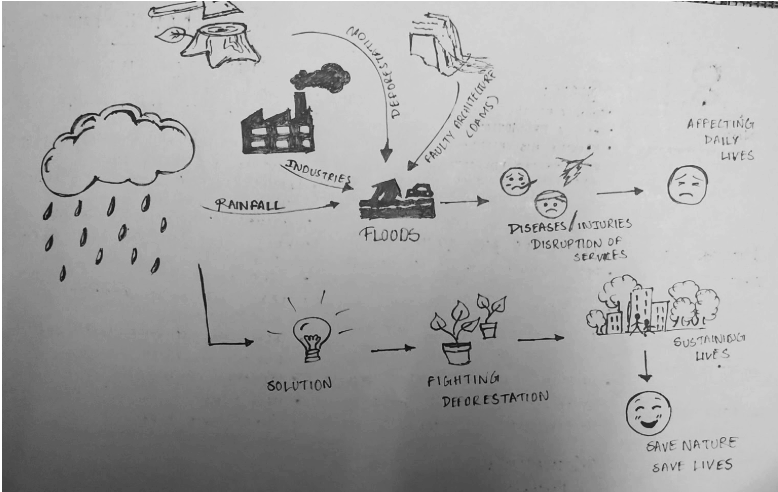
\includegraphics[width=\linewidth]{journeymap.png}
	    \caption{Journey Map from adverse effects of floods \& deforestation to a greener and sustainable future.}
	    \label{fig:map}
    \end{figure}

Figure \ref{fig:map}
Flood-influencing factors as independent variables are essential to generate a flood susceptibility map (Liu \& De Smedt, 2005). Kia et al. (2012) argued that the contributing parameters used for specific study areas may have no impact in other regions, therefore variable selection should be case-specific. In such case, scarcity of data can limit the the number of models that can be used to identify flood risk zones. A possible solution to this can be the use of GIS (Geographical Information System) based models to provide a more accurate prediction.  GIS coupled with various models have been used before to create flood susceptibility maps. Out of these ANNs (Artificial Neural Netwoks) and SVMs (State Vector Machines) have shown promise in accuracy of prediction. Depending onthe region in focus, and the data available we will use one of the models to accurately identify flood risk regions. Analysing the factors afecting the floods using the learning vector quantization process(LVQ) will help us identify the major contributing factor. 
We will use statistical data based on various factors, maps and images. The datasets can either be real-time data collected from Synthetic Aperture Radar(SAR) or historical data recorded before.   

	\section*{Feasibility:}
		The risk of coastal flooding is increasing as a result of deforestation, untimely and torrential rains, sea level rise etc. In the event of floods occurring, a large amount of damage can be curbed if we have a model that could predict floods in advance. To avoid devastating consequences which have a major impact on economic and financial conditions of the city, our system aims to provide maximum accuracy in alerting target regions about the forthcoming disasters. This model can be extended for different locations in the future.
Not many ways we use today for addressing environmental challenges employ evolving and proven technologies like Artificial Intelligence and Machine Learning visible in inaccurate results (e.g. erroneous weather predictions etc).  The methods which are currently being used to address floods and other environmental challenges have a high degree of uncertainty associated with them.
With a reliable flood prediction model in place, government authorities in the targeted regions will be alerted about the impending floods in advance and will hence be able to evacuate the people living there and minimize other damages caused by the floods. Information regarding the range of the region which will be affected will enable the authorities to employ relief procedures accordingly.

        \section*{References:}
        \begin{itemize}
        \item \href{https://www.thestar.com.my/opinion/letters/2014/11/08/deforestation-the-cause-of-flood}{Deforestation the cause of floods.}
        \item \url{http://india-water.gov.in/ffs/}
        \item \href{https://ai.googleblog.com/2019/03/a-summary-of-google-flood-forecasting.html}{Google Flood Forecasting}
        \item Flood Prediction Using Machine Learning Models: Literature Review Amir Mosavi, Pinar                                    Ozturk, and Kwok-wing Chau.
             \\Link: \url{https://arxiv.org/ftp/arxiv/papers/1908/1908.02781.pdf}
         \end{itemize}

\end{document}